\chapter{Methods: Evaluating Motion Patterns}
\label{ch:mopa}

In the previous chapter, we described the methods we use to mitigate the positional effects of motion in rs-fMRI sequences. We briefly discuss how the registered sequences were evaluated with respect to gold standard usability criteria. Here, we expand on our analysis of the motion extracted from the sequences.

\section{Measuring Motion Patterns}

While the Power et al. usability thresholds for the FD and DVARs metrics quantify the volume-to-volume motion well, they do not quantify the overall motion contained in the image sequence. The FD and DVARs metrics, as well as other imaging metrics, can be used to compare every volume in an image sequence to every other volume in the image sequence to quantify global motion more effectively. As the FD and DVARs metrics have been discussed previously, we focus in this section on two other image metrics: the Dice coefficient and the mutual information. These five metrics were applied to each whole sequence to measure patient motion and image signal consistency throughout the entire scan.

\subsection{Dice Coefficient}

The Dice coefficient was proposed by Lee R. Dice in 1945 \cite{Dice1945}. Dice examined several existing metrics for measuring association, and finding them lacking, proposed his own ``coincidence index''. His coincidence index measures the association between a set of samples $a$ where condition $A$ is true and a set of samples $b$ where condition $B$ is true:

\begin{equation}
Index = \frac{2h}{a+b}
\end{equation}

In this equation, $h$ represents the number of samples where both conditions $A$ and $B$ are true. His index can take on any value between 1.0 and 0.0 such that a value of 1.0 means that conditions $A$ and $B$ are true for all samples. Similarly, a value of 0.0 means that conditions $A$ and $B$ are never both true for any sample. While this index is a count of samples that meet both conditions and not an actual probability, Dice suggests that the chi-squared test can be used to determine if the combinations of conditions in the samples from a set of data are meaningful or due to random chance. 

Many medical imaging researchers have adapted the Dice coefficient to measure the overlap between pairs of images. 
Zijdenbos et al. trained an artificial neural network to semiautomatically segment brain MRIs and compared the generated segmentations to manual segmentations using the Dice coefficient \cite{Zijdenbos1994}.
Zou et al. used the Dice similarity coefficient in their analysis of the reproducibility of manually segmented MRIs and the accuracy of automatic segmentations of the same images for prostate and brain tumor datasets \cite{Zou2004}. 
Liao et al. used it to measure the accuracy of a volume registration framework for aligning manual segmentations of multiple organs in fetal images \cite{Liao2016}. Bharatha et al. performed a study on pre- and intra-operative images of the prostate. They segmented the images and used the segmentations to generate deformable finite element models of the organs. They compared the registered segmentations and finite element models using the Dice coefficient \cite{Bharatha2001}.

It should be noted that the Dice coefficient, as used in these contexts, is a measure of similarity of items from two categories where each item belongs to one of two binary classes. The two classes of interest in the case of rs-fMRIs are ``brain'' or ``not brain''. Medical images do not naturally have binary values. All studies mentioned in the previous paragraph required a domain expert to manually segment each image that was analyzed using the Dice coefficient. The manually segmented images are considered the gold standard to which automatic segmentations or registered images can be compared. 

The images in our dataset have been manually curated to remove the skull and other anatomical features outside of it, but the images still contain a continuous range of voxel intensity values. The Dice coefficient cannot be directly applied to these image sequences, even though each voxel only belongs to one of two classes. The volumes first must undergo thresholding to create binary images to clearly separate the brain and the background for computational purposes. We use Otsu thresholding to accomplish this task. 

Otsu thresholding divides the contents of an image into two binary classes based on the histogram of voxel intensity values. It assumes that the classes are represented in the histogram by separable peaks. It separates the peaks by finding the separation threshold with the best separation between classes. In its original form, Otsu thresholding exhaustively searches the space of all possible thresholds. For each threshold, it calculates the within-class variance and between-class variance for the pair of classes separated by the current threshold option. The ideal threshold is the one that produces the minimal within-class variance and the maximal between-class variance. The ideal threshold is then used to convert the original image into a binary image volume where background voxels have a value of zero, and voxels in the brain have a value of one. The binarized image volumes can be compared to each other using the Dice coefficient. 

In cases where a good Otsu thresholded binary image cannot be obtained, other similarity metrics such as mutual information and cross-correlation should be used instead.

\subsection{Mutual Information}

The earliest description of mutual information was written in the context of mathematical theories behind networked communication \cite{Shannon1948}. Mutual information is a measure of the amount of information shared between two signals $X$ and $Y$. Specifically, mutual information measures how the joint distribution of the two signals compares to the marginal distribution of each signal \cite{Li1990}. It is a more general measure of dependence than correlation, which is limited to measuring linear dependence via a comparison of the marginal distributions. In terms of information theory, mutual information is represented as

\begin{equation}
\label{ch4:eq:mi_01}
MI(X, Y) = H(X) + H(Y) - H(XY)
\end{equation}

\noindent where $H(X)$ is the entropy of signal $X$

\begin{equation}
\label{ch4:eq:mi_02}
H(X) = - \sum_{x \in X} p_x log(p_x) 
\end{equation}

\noindent where $p_x$ is the marginal distribution of the signal $X$. Substituting $y$ for $x$ in this equation produces $H(Y)$, the marginal entropy of the signal $Y$. Similarly, $H(XY)$ is the joint entropy of signals $X$ and $Y$ given the known signals $X$ and $Y$

\begin{equation}
\label{ch4:eq:mi_03}
H(XY) = - \sum_{x \in X, y \in Y} p_{xy} log (p_{xy}).
\end{equation}

It is worth noting that since the two signals of interest are registered images, $x$ and $y$ refer to voxel locations in the same image space. Substituting Equations \ref{ch4:eq:mi_02} and \ref{ch4:eq:mi_03} in Equation \ref{ch4:eq:mi_01} produces the following

\begin{equation}
\label{ch4:eq:mi_04}
\begin{split}
MI(X, Y) & = - \sum_{x \in X} p_x log(p_x) - \sum_{y \in Y} p_y log(p_y) + \sum_{x \in X, y \in Y} p_{xy} log (p_{xy}) \\
 & = \sum_{x \in X, y \in Y} p_{xy} log p_{xy} - \left( \sum_{x \in X} p_x log(p_x) + \sum_{y \in Y} p_y log(p_y) \right) \\
\end{split}
\end{equation}

\noindent In the case where signals $X$ and $Y$ are independent, Equation \ref{ch4:eq:mi_04} can be simplified to

\begin{equation}
\label{ch4:eq:mi_05}
\begin{split}
MI(X, Y) & = \sum_{x \in X, y \in Y} p_{xy} log (p_{xy}) - \left( \sum_{x \in X} \sum_{y \in Y} p_{xy} log(p_x p_y) \right) \\
 & = \sum_{x \in X, y \in Y} p_{xy} log \left( \frac{p_{xy}}{p_x p_y} \right) \\
\end{split}
\end{equation} 

Mutual information can be used to determine how the distribution of amplitudes in one signal relates to the distribution of another signal. It is commonly used in the medical imaging domain to objectively compare images of the same tissue taken using different modalities. For example, a computed tomography (CT) scan of a patient's abdomen contains different information about each tissue types' material properties than an MRI of the same organs. Some tissue types may appear similar in one of these modalities but drastically different in the other. Combining the information about a tissue's material properties gained from both imaging modalities provides more information than could be gained from either modality independently. (In other words, the resulting information is greater than the sum of its parts.)

Even though the rs-fMRIs in our study are all obtained using the same imaging modality, the spin history effects of patient motion can impact the recorded signal such that small changes in the recorded BOLD signals are difficult to distinguish from noise. We choose to use mutual information to quantify to BOLD signal information across the entire image sequence.

\subsection{Implementation: Tools and Libraries}

To calculate metrics, we used several existing tools and libraries. When no existing tool could be found, functions were implemented manually in Python3. 

For the Dice coefficient calculation, we first had to create a binary version of each image volume. To binarize the image volumes, we used Simple ITK's Otsu thresholding function. The binary images were then passed to a manually implemented function to calculate the Dice coefficient.

The correlation ratio between each possible pair of volumes in the sequence was calculated using bash and FLIRT (FMRIB’s Linear Image Registration Tool) \cite{Jenkinson2001} \cite{Jenkinson2002}. We then used the average and standard deviation of the correlation ratio distribution of each image to compare the images.

The mutual information calculation was implemented in two steps. The first step was to create a function that computes the joint histogram of the voxel value distributions between the two image volumes. This histogram was fed to a second function that converts the histogram counts to probabilities and calculates the mutual information value. 

%--------------------------------------------------------------------------

\section{Patient Classification Using Motion Patterns} 

%Machine learning techniques can be used to classify images as belonging to different groups, but many of these techniques use difficult-to-interpret ``black box'' logic. In some cases, examining the logic behind a classification reveals patterns in a dataset that a human missed, but a computer detected. These patterns can help improve human classification of the images, but they may also be based on artifacts that were not filtered out during preprocessing.

We suggest that patient movement patterns are specific to certain age groups. For example, fetal patients live suspended in amniotic fluid and, as such, are subject to different physical constraints than patients in other age groups. Neonatal patients are often scanned using a ``feed and bundle'' protocol, which often results in them sleeping through the scan. However, neonatal patients sometimes wake up during the scan, and the way a baby woken from a nap moves is different from how a fidgety preadolescent moves.

There is also a chance that patients within the same age group move differently, possibly due to their cognitive state. Preadolescents who have ADHD likely become bored and fidgety in the MR scanner at different rates than their non-ADHD counterparts. Adults who have dementia may have more difficulty remaining still for the duration of a scan than adults from similar demographics with no dementia.

These patterns are essentially signals specific to different categories of patients. Machine learning techniques are useful for identifying patterns in signals from different sources. In addition to the motion metrics identified in the previous section, we also use demographic data as features for our machine learning models. 

The goal of applying machine learning to identify population-level motion patterns lends itself well to unsupervised machine learning techniques. Unsupervised learning techniques combine samples from a population into groups based on the patterns in their features. They do not use information about any known groups in the population to inform their classification processes. In this section, we discuss several different unsupervised machine learning techniques used to measure degrees of association within subgroups of a data set.

\subsection{K-means Clustering}

\begin{figure}
\centering
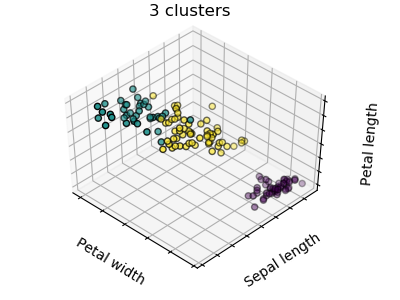
\includegraphics[width=.5\textwidth]{4/kmeans-example.png}
\caption{An example of $k$-means clustering performed on the Iris data set. The results of the algorithm are highly dependent on the number of clusters specified.}
\label{ch4:fig:kmeans}
\end{figure}

K-means clustering divides a group of data samples with $n$ features into $k$ groups based on each sample's distance from the average value of the group \cite{Hartigan1979}, \cite{macqueen1967}. In k-means clustering, the features of a set of data are viewed as the locations of each data sample in \textit{n}-dimensional space. In this space, \textit{k} cluster centroids are initially distributed. The distribution pattern can place the centroids either randomly between data samples or using randomly selected data points.

After the locations of the cluster centroids are initialized, the distance between each sample and each centroid is calculated. Each sample is assigned to the cluster represented by the centroid closest to it. Once the clusters are defined, the location of the centroid of each cluster is recalculated. The new centroid location is the mean of the locations of all samples in its cluster. The distance between each sample and each cluster centroid is recalculated and the samples are reassigned to their closest cluster centroid. Then the centroid of each cluster is recalculated. This process continues until a stopping criterion is fulfilled. With most unsupervised machine learning methods, the stopping criterion is that the classifications of the model do not change for a certain number of iterations. However, a maximum number of iterations is imposed on the learning process to prevent a model from running indefinitely. As a result, it is possible for a model to ``time out'' before reaching a stable state.

There are many variations of k-means clustering. For example, k-medians follows the same steps as k-means, but uses the median of the known data points in a cluster as the new centroid for that cluster \cite{Juan1998}. Another variation called k-medoids uses the data point closest to the center of the cluster as the new cluster centroid rather than a descriptive statistic of the cluster \cite{Kaufman1987}.

One of the major limitations of k-means clustering is that the number of clusters must be given to the model. It is difficult to know how many clusters are needed to adequately represent subgroups within a data set. If too many clusters are used, the groups identified by the algorithm are more granular than they should be; however, using too few clusters produces large groups that mask distinct subgroups. An example of k-means clustering as applied to the Iris data set can be seen in Figure \ref{ch4:fig:kmeans} \cite{Varoquaux2019}. The results of the clustering are dependent on the number of clusters specified as well as the points used to initialize the algorithm.


\subsection{Spectral Clustering}

While spectral clustering is related to k-means clustering, it approaches the problem of identifying associations in a group of data from a different perspective. Spectral clustering treats each data point in a sample as a node in a graph. The connections between data points are characterized by the adjacency matrix and the degree matrix of the graph. These two matrices are used to calculate the Laplacian matrix of the graph, whose properties are used to identify clusters. All three matrices are $n$x$n$ matrices, where $n$ is the number of data points in the sample. 

Herein, we discuss spectral clustering when the data can be represented using a simple graph. As such, certain mathematical shortcuts can be employed to simplify certain computations. A more general mathematical approach has been discussed by Ng, Jordan, and Weiss \cite{Ng2002}.

The adjacency matrix specifies the strength of the connections between the nodes represented by the rows and columns of the matrix. For data that does not begin in graph form, algorithms such as k-nearest neighbors can be used to generate the adjacency matrix. In the adjacency matrix, each entry $i, j$ contains the weight of the connection between node $i$ and node $j$. If the edges are unweighted, the value of the entry is either 0 or 1. If the graph is undirected, the value of entry $i, j$ is the same as the value of entry $j, i$. All entries where $i=j$ should be 0 unless node $i$ has a self-loop.

The degree matrix is a diagonal matrix that represents the number of edges connected to each node. If the graph is directed, the directionality of the degree matrix must be specified: a directed connection from node $a$ to node $b$ contributes to the count for node $a$ if the degree matrix counts the number of edges that begin at each node (outdegree), but contributes to the count for node $b$ if the degree matrix counts the number of terminating edges at each node (indegree). In the case of an undirected graph, the connections include all edges that begin or terminate at a node. To summarize, in a directed graph, each edge contributes to only one node count, while in an undirected graph, each edge contributes to both nodes.

The adjacency matrix and the degree matrix are used together to construct the Laplacian matrix of the graph. This calculation of the normal Laplacian for a simple graph (undirected and containing no loops) is straightforward: the adjacency matrix is subtracted from the degree matrix. The resulting matrix has the following properties:
\begin{itemize}
\item The diagonals are the number of connections per node less the number of self-connections
\item All off-diagonal values are the negative of the weight connecting node $i$ to node $j$.
\end{itemize}
It is important to note that if the graph in question contains loops or is directional, other methods must be used to calculate the Laplacian matrix. 

The Laplacian matrix can be used to explore many properties of a graph. In particular, the eigenvalues of the Laplacian matrix are informative about the number of connected components in the graph. Connected components are areas of the network that are connected to each other but not anything outside that component. Each connected component is not its own cluster, though: the connected components could be large and contain smaller sets of connected nodes that are good options for clusters.

Several steps are used to determine the number of clusters in the graph. First, the eigenvalues of the Laplacian matrix are sorted in increasing order. The number of zero-valued eigenvalues is the number of connected components in the graph. Eigenvalues close to zero suggest weak edges preventing some connected components from being two separate components. Manually examining these eigenvalues before performing spectral clustering can be informative about the number of clusters to create: the number of values below the first large gap between the eigenvalues is the number of clusters, $k$. The eigenvectors associated with these $k$ eigenvalues are used as a lower-dimensional representation of the data in the graph. Performing $k$-means clustering on this data produces the labels for the clusters within the data that are not linearly separable otherwise.

\begin{figure}
\centering
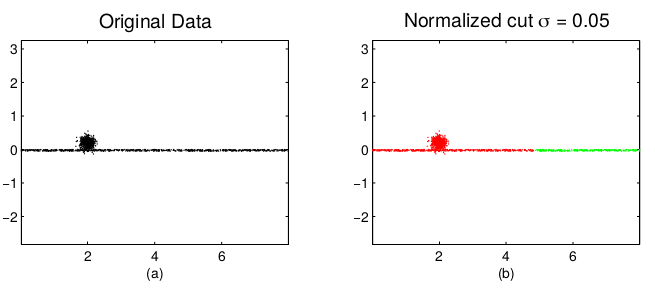
\includegraphics[width=.75\textwidth]{4/spectral_clustering_limitation.png}
\caption{(a) Two different distributions, a 2D Gaussian density and a thin horizontal rectangle are difficult to separate (b) due to their overlap and the penalties built into the cost function of the spectral clustering algorithm. From \cite{Nadler2007}.}
\label{ch4:fig:spect-clust-lim-01}
\end{figure}

The limitations of spectral clustering are strongly related to the process of remapping the data to a lower-dimensional space.  When reducing the number of features used to represent a data set, information about that data set is inherently lost. The missing information can make separating classes in the lower dimensional data significantly more difficult, if not impossible. Consider the following two cases: a case where two classes overlap and a case where three classes are unevenly represented in the data.

In cases where two seemingly obvious clusters overlap, the clustering algorithm may be unable to accurately identify them due to the mathematical penalties imposed on separating points in the feature space. An example of this problem as described by Nadler and Galun can be seen in Figure \ref{ch4:fig:spect-clust-lim-01} \cite{Nadler2007}. The two distinct groups are the small 2D Gaussian density and the horizontal rectangle. The spectral clustering algorithm (in this case, the normalized cut algorithm) is unable to separate the groups because the degree of overlap between the Gaussian density and the rectangle is greater than the height of the rectangle. It is more cost-effective for the algorithm to make a vertical cut to divide the rectangle in two than to cut the Gaussian density away from the rectangle.

Uneven distributions of data classes can severely impact spectral clustering results. Consider the case where a data set contains one highly populated class with a wide variation in its data features and two less populated classes with less variation in their data features. The scale of the large, highly populated class can overshadow the smaller classes: if the three most significant eigenvectors are more related to the large class than the smaller classes, the algorithm cannot differentiate between the two smaller classes.

\subsection{Agglomerative Clustering}

\begin{figure}
\centering
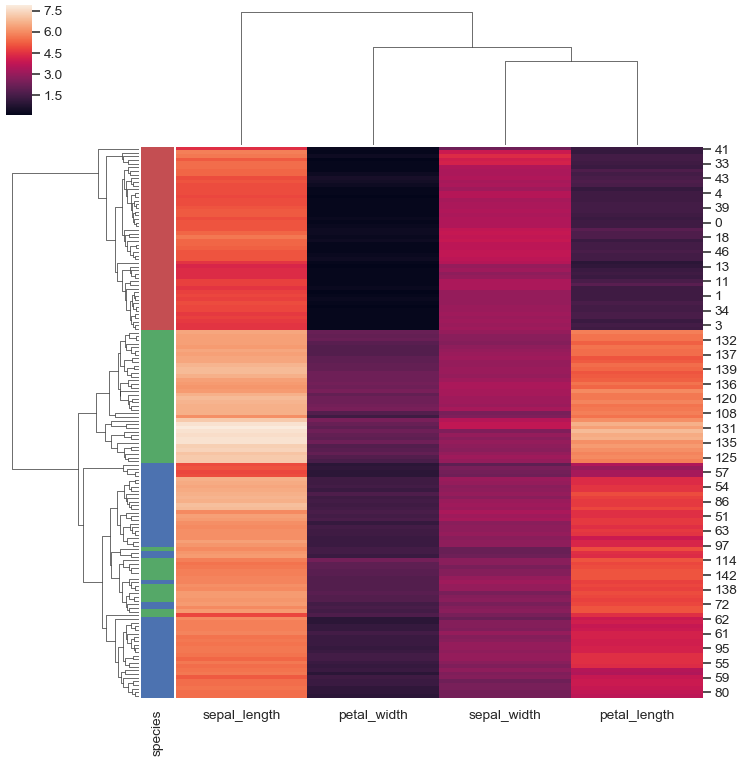
\includegraphics[width=.5\textwidth]{4/clustermap-example.png}
\caption{An example of agglomerative clustering on the Iris data set plotted using \textbf{seaborn}'s \textbf{clustermap} function.}
\label{ch4:fig:agg}
\end{figure}

Agglomerative clustering is a specific type of hierarchical clustering that builds a tree of similarities between data samples from the ``bottom up'' \cite{Ward1963}. The data samples in agglomerative clustering are also viewed as distinct points in $n$-dimensional space, but the number of groups to identify is not specified. 

First, the distance from every data sample to every other data sample is calculated. The two data points that are closest together in terms of a similarity metric are combined into a single cluster. In the relationship tree representing the similarities between all data samples, a node is created and the joined data points are connected to that node. That node or cluster is treated as an intermediate data sample. The distance from the new ``data sample'' to every other data sample is calculated, and the two closest data samples are again combined into another intermediate sample. A node representing the new cluster is added to the relationship tree and the data sample or samples merged into the cluster are connected to the node. The process of combining data points into clusters based on similarity to other data points terminates when all data points and clusters have been combined. 

The results of agglomerative clustering can be interpreted by traversing the relationship tree. The relationship tree recorded the history of which nodes were merged into which clusters at each stage. Due to the nature of agglomerative clustering, these stages can be viewed as distinct levels in the tree. The granularity of the clusters can be explored beginning at the final node (the root) of the tree. At the top level, there is only one cluster, but at the second to last level of the tree, there will be two clusters; at the third level, there will be three clusters, and so on. How each cluster grew can reveal information about the relationships between the data samples within that cluster.

Agglomerative clustering also lends itself well to visualization via heatmap. The heatmap allows the researcher to see the distribution of feature values across the dataset and across visually prominent clusters. The Python library \textbf{seaborn} has a function called \textbf{clustermap}, which both performs agglomerative clustering and shows the resulting trees in a structured heatmap. An example of agglomerative clustering from the \textbf{seaborn} documentation in which the clustering was applied to the Iris data set can be seen in  Figure \ref{ch4:fig:agg} \cite{Waskom2018}. Each column represents a feature and each row represents a single sample. The colorbar in the top left of the figure shows that lighter colors in each cell represent higher values. The dendrogram along the top of the heatmap shows the distance between each feature. The dendrogram along the left of the heatmap shows the distance between each data sample and the data sample most similar to it. The column immediately to the right of this dendrogram shows the known class (species) for each data sample. The class labels in conjunction with the dendrogram of the data samples show the distinct groups present in the data which were identified using agglomerative clustering. 

\subsection{Visualizing Clustering Results} 

The results of unsupervised clustering algorithms can be visualized to illustrate how the computer chose each group of samples. Depending on the number of features $n$ for each data sample, a dimensionality reduction method may be needed to transform the location of the data sample in $n$-dimensional feature space to a more easily visualized 2-dimensional or 3-dimensional space. The three-dimensionality reduction methods we consider are principal component analysis (PCA), T-distributed stochastic neighbor embedding (t-SNE), and uniform manifold approximation and projection (UMAP).

\textbf{PCA}. Principle component analysis is a multivariate statistical technique that can be used to transform a set of variables with some degree of intercorrelation into a set of new, independent, orthogonal variables \cite{Abdi2010}. These variables are called principal components of the data set. The principal components are ordered with respect to the amount of variance in the data set that can be projected onto each component. In general, PCA fits an $p$-dimensional ellipsoid to a data set with $n$ features such that $p < n$. Each axis of the ellipsoid represents a single principal component. The first two or three principal components can be used to plot the results of a clustering algorithm in 2D or 3D space.

It is important to note that prior to the application of PCA, the data must be normalized. Normalizing the data allows different features to be compared on the same scale.

\textbf{t-SNE}. T-distributed stochastic neighbor embedding (t-SNE) was developed by Maaten and Hilton to perform nonlinear dimensionality reduction for visualizing high-dimensional data in a 2D or 3D space \cite{Maaten2008}. The algorithm first constructs a distribution of the high-dimensional data to measure the pairwise similarity of all data points. It also constructs a second distribution to measure the pairwise similarity of the data points in the lower dimensional space. Then, it performs gradient descent to minimize the difference between the two distributions as measured by the Kullback-Leibler divergence. At each iteration of the gradient descent, the distribution of points in the lower dimensional space is modified. The algorithm converges when the distribution of pairwise similarities between data points in the lower dimensional space most closely matches the corresponding distribution in the original high-dimensional space.

t-SNE is a computationally expensive technique with a complexity of $O(N^2)$ where $N$ is the number of data points. For this reason, it is recommended that data with more than 50 features undergoes another form of dimensionality reduction before t-SNE is applied to a data set. Even when this recommendation is not followed, the lower-dimensional data produced using t-SNE lacks the interpretability of PCA data: the resulting dimensions have no interpretable meaning.

\textbf{UMAP}. Uniform manifold approximation and projection (UMAP) was proposed as an alternative to t-SNE \cite{McInnes2018}. Rather than build a pairwise similarity distribution, UMAP uses topological representations of the data. For each point $x_i$, the distances between $x_i$ and its $k$ nearest neighbors are measured and normalized by the distance between $x_i$ and the $k$th neighbor. These collections of distances around each point are local manifolds. The local manifolds are combined into the same global manifold using fuzzy simplicial sets. After the global of the data is known, it is used to determine where data points must lie in a lower-dimensional space so that they both adhere to the known manifold topology and retain the distance metrics from their $k$ nearest neighbors. The topology of the lower dimensional manifold is adjusted iteratively to minimize the cross-entropy between the higher dimensional representation and the lower dimension representation. In practice, UMAP treats each data point as a node in a weighted graph. It first determines each point's $k$ nearest neighbors, calculates the distances between them, and then computes a version of that topology in a lower-dimensional space.

UMAP was developed under the belief that local structure is more important than global structure. It learns structures in a data set, even when the local structures can only be attributed to noise. It is not suitable for use in small, noisy data sets or in large data sets with only global (not local) structure. Figures produced using UMAP-reduced data should be interpreted with care: they could contain spurious structures from the data sample and not the target population. Additionally, UMAP is similar to t-SNE in that the dimensions produced by UMAP were generated nonlinearly and contain no true meaning. 

\begin{figure}
\centering
\begin{subfigure}{0.3\textwidth}
  \centering
  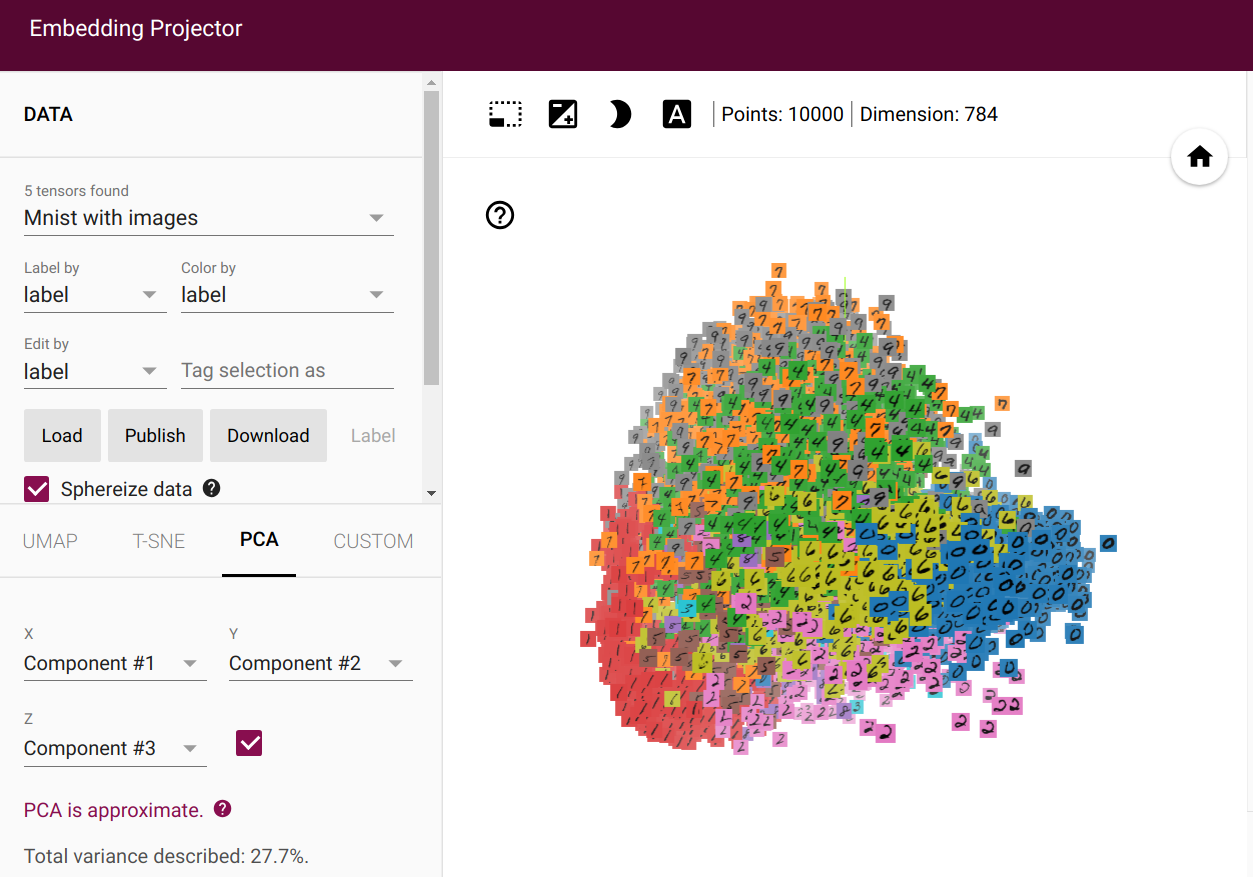
\includegraphics[width=1.0\textwidth]{4/pca.png}
  \caption{PCA}
\end{subfigure}
\hspace{0.02\textwidth}
\begin{subfigure}{0.3\textwidth}
  \centering
  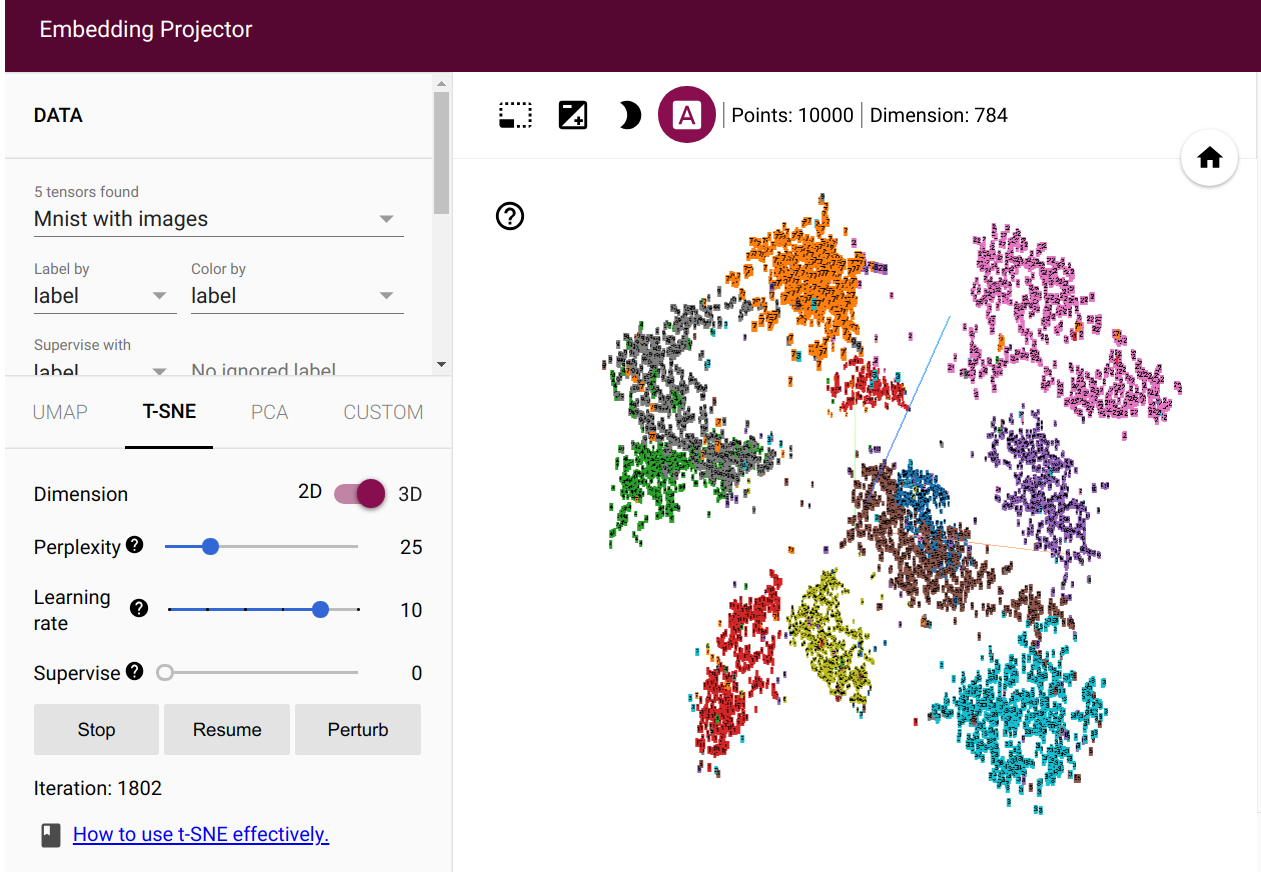
\includegraphics[width=1.\textwidth]{4/tsne.png}
  \caption{t-SNE}
\end{subfigure}
\hspace{0.02\textwidth}
\begin{subfigure}{0.3\textwidth}
  \centering
  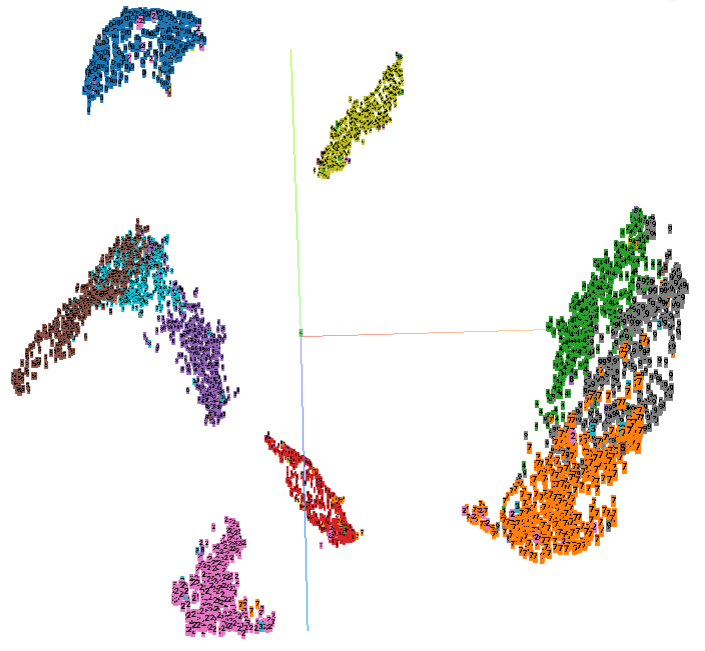
\includegraphics[width=1.0\textwidth]{4/umap.png}
  \caption{UMAP}
\end{subfigure}
\caption{Visualization of MNIST data in 3D via TensorFlow Projector as generated using PCA, t-SNE, and UMAP dimensionality reduction techniques.}
\label{ch4:fig:data-viz}
\end{figure}

We performed a preliminary comparison of PCA, t-SNE, and UMAP for visualizing high dimensional data using TensorFlow's Projector tool \cite{TFProjector}. This tool is a web interface for visualizing high dimensional data from either built-in data sets or data sets uploaded by the user. It supports all three of the dimensionality reduction methods discussed previously in this section as well as a customizable projection of the entire data set to two or three feature vectors. The PCA, t-SNE, and UMAP visualizations of the popular MNIST handwriting data set can be seen in Figure \ref{ch4:fig:data-viz}. 